\chapter{Experiments}
\label{Experiments}
\thispagestyle{empty}
In this chapter, we present the results of our experiments. 
First, we talk about the design of the reference trajectory.
Then, we show the performances obtained by the controller optimized with POIS, train starting from human-crafted parameters. Afterwards, we will discuss the experimental choices made about the PPO in trying to improve the lap-time performance.
At the end, we will show all the hyperparameters chosen for this thesis project.


In this chapter, we present the results of the application of the algorithms described in Chapter \ref{Methods} on the TORCS simulator. After giving information about how expert demonstrations are gathered and about the simulator itself.
We will show the application of our controller as a method to follow a reference trajectory and how it can be optimized by using Reinforcement Learning algorithms. Then we will discuss about the application of policy improving
algorithms and about the one policy approach

\section{Expert demonstrations and Reference Trajectory}

We choose as track over which do the experiments the TORCS track called \textit{Forza}, which takes inspiration from the real-world \textit{Monza} track. Demonstrations are collected by a team of non-expert human drivers each of one
played on the simulator recording its best laps. Then, the reference trajectory is chosen to be the lap with lowest lap time that never goes out of track (i.e., cutting turns). That's because the TORCS track range sensors returns
an invalid value as soon as the car goes out of track and then those data cannot be used. The chosen reference trajectory is shown in Figure \ref{fig:ref_traj} and the lap time is equal to $71.99s$. Figure \ref{fig:ref_traj} also shows numbered curves
that will be used as reference in the next plots.
The reference trajectory is a collection of state-action pairs collected with a sampling frequency of $100Hz.$


\begin{figure}[H]
 \centering
  \captionsetup{width=12cm}
  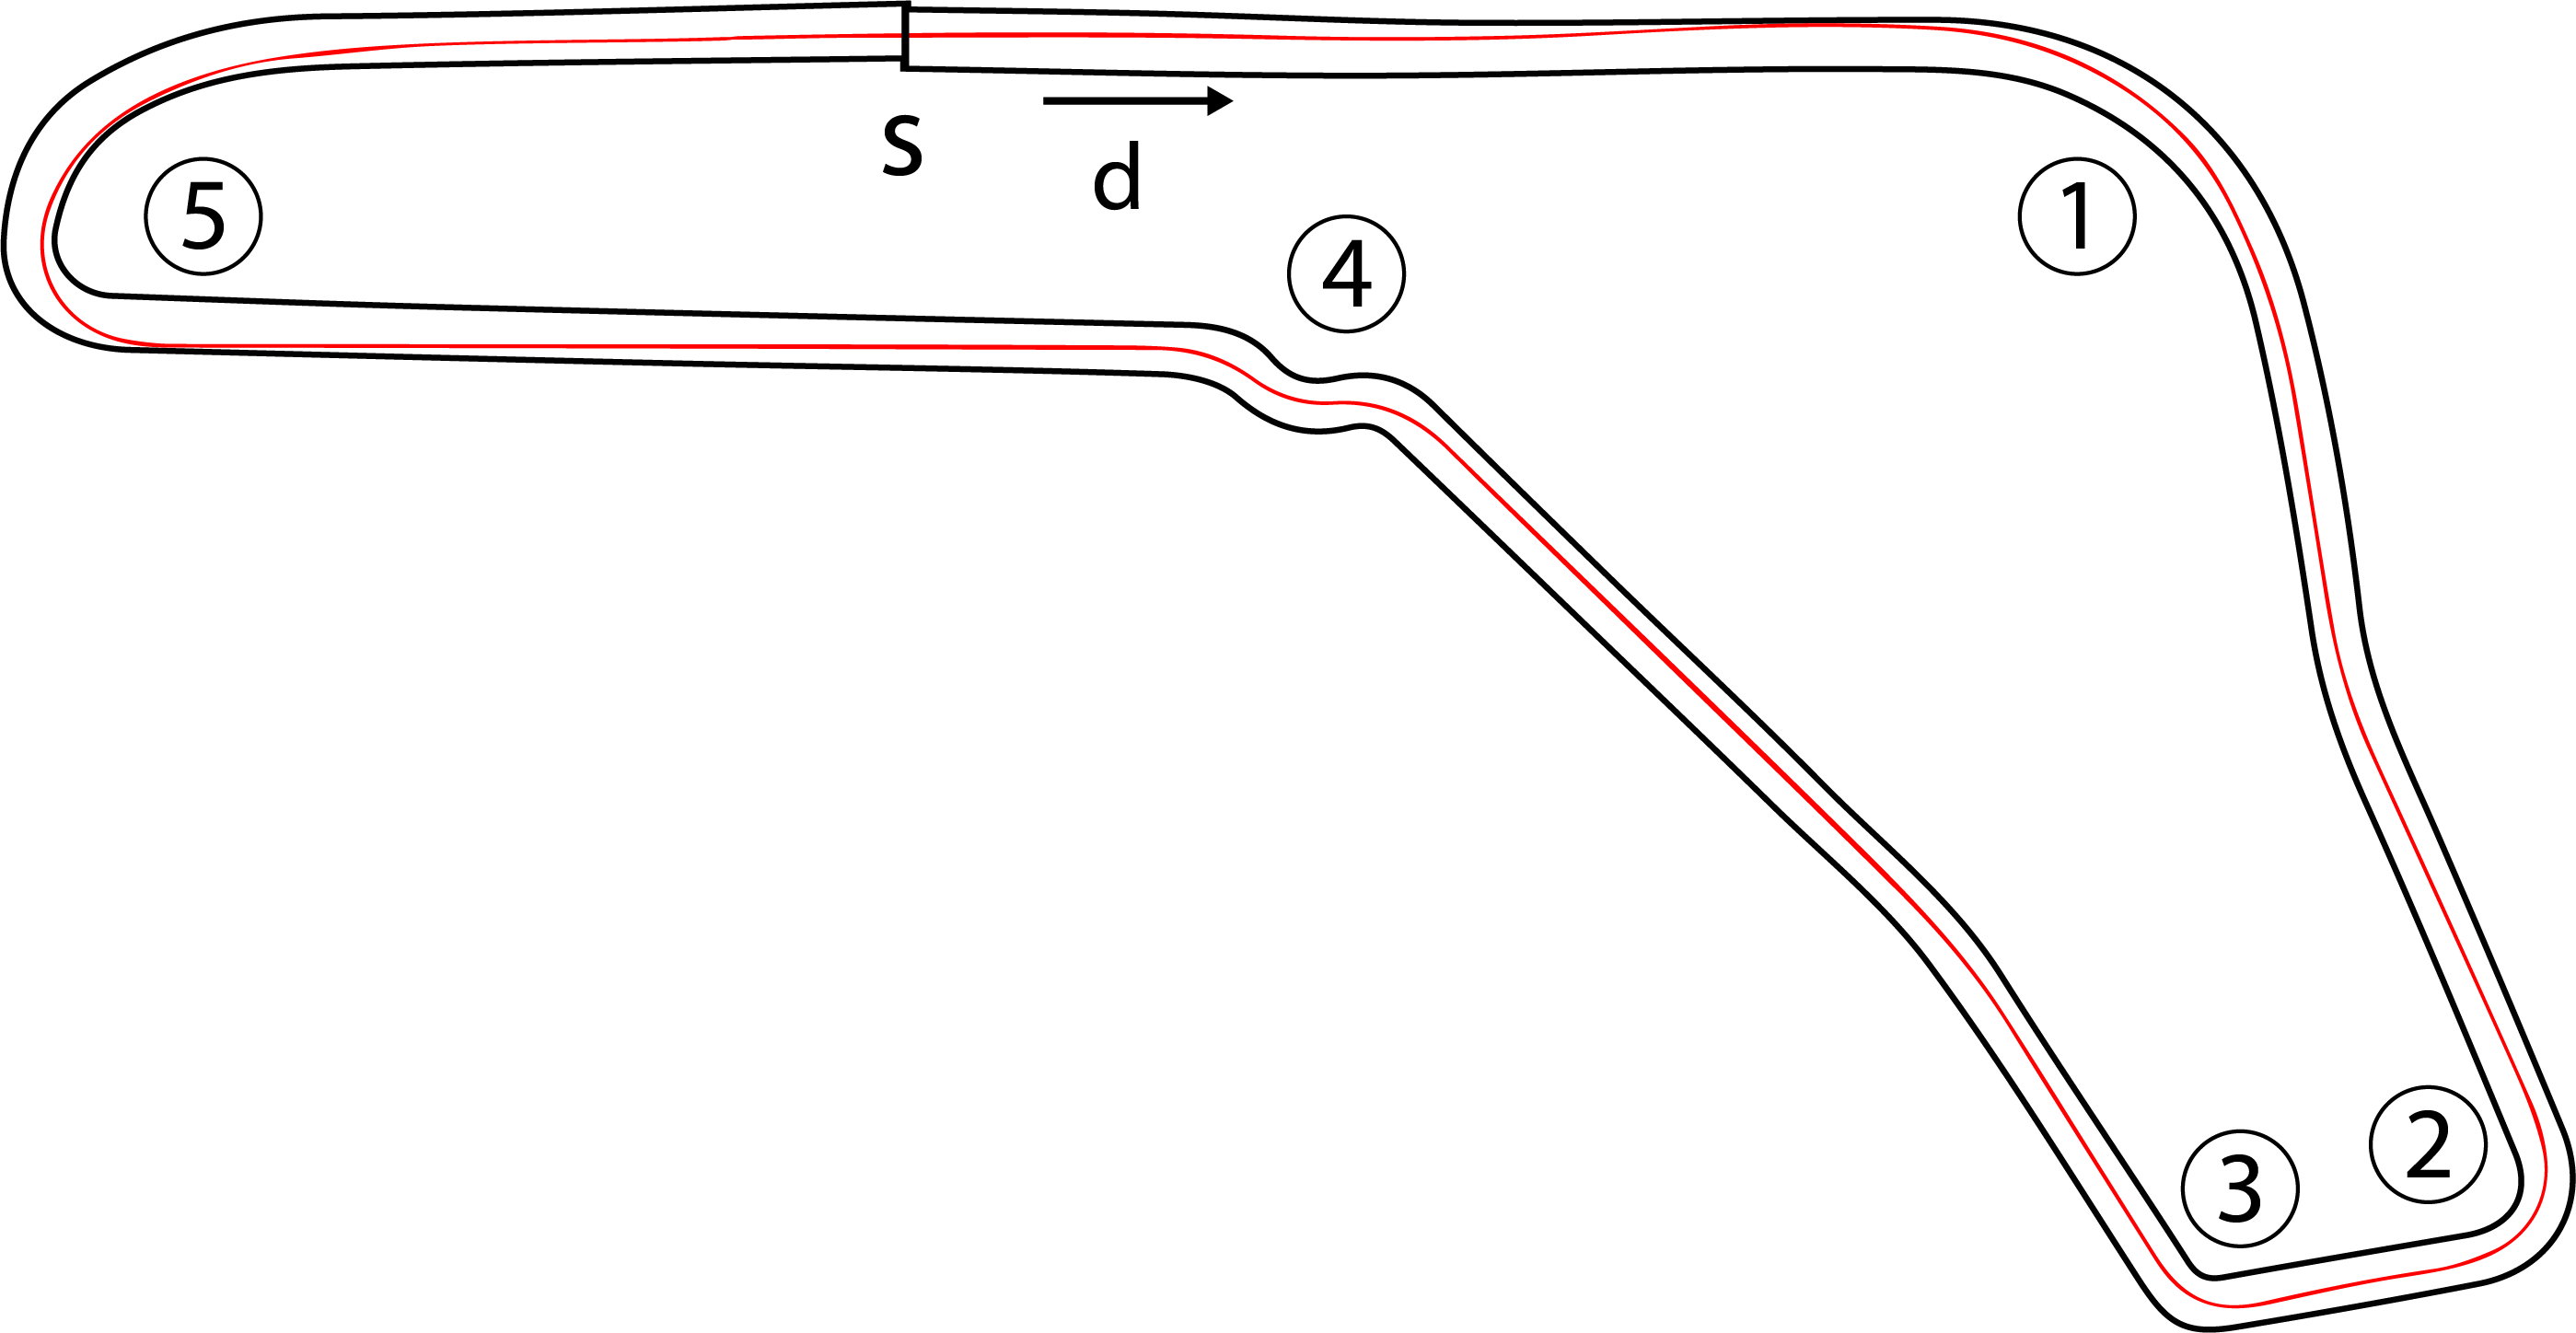
\includegraphics[width=12cm]{./img/ref_traj}
  \caption{Reference trajectory, where $s$ is the starting point and $d$ is the driving direction.}
   \label{fig:ref_traj}
\end{figure}

After the expert demonstrations are collected and the reference trajectory has been defined, it is possible to apply the algorithms described in Chatper \ref{Methods}. First of all, we discuss the two-step framework which consists in learning a policy
that follows the reference trajectory and another one that improves the lap time. This framework is formulated in Sections \ref{ref_follow}, and \ref{ref_improve} for policy following and improvement respectively. Then, we will discuss about the direct approach which consists in learning a single policy that learns to drive by using human demonstrations.

In the next sections, we will show the results obtained for each algorithm.

\section{Two-step Framework}
As described in Chapter 5, for the two step framework we used the algorithms POIS for the first stage and PPO for the second one. Before to apply POIS on the controller we inizialied the controller parameters $\boldsymbol {\omega}_0$ manually with a trial and error approach. This is done to speed up the initial learning phase of the algorithms, indeed, we run POIS over a set of controller's parameters that allows the controller to complete a lap.
Even if the human-initialized controller was able to complete a lap, it has the main limitation that the car during tight curves goes a bit out of track. As we will see, the optimization made by the RL algorithm is able to solve
this issue.

In this section, we will show the result of the optimization policy via POIS and of the obtained estimation of the optimal rule-based policy $\psi^*_{\boldsymbol \omega}$ , i.e. $\hat{\psi^*}_{\boldsymbol \omega}$.
\subsection{POIS}
We run POIS with the parameter vector $\boldsymbol {\omega}_0$ shown in Table \ref{tab:omega_0}. Every iteration consists in a batch of $200$ trajectories. Since the the environment is deterministic, each trajectory is obtained by sampling from the hyper-policy a parameter vector for each trajectory. The reward function we used is $r_{\text{space}}$ (Eq. \ref{eq:r_space}). In order to avoid the agent to go out of track we used a negative penalty equal to $-2000$ that is added to the reward signal. Figure \ref{fig:poislearning} depicts the mean reward of the $200$ trajectories: on the $x$ axis we have the iterations made by the algorithm, on the $y$ is the reward function. From this plot we notice that the algorithm converges around $8000$ iterations.

\begin{table}[H]

\centering
\begin{tabular}{|c|c|}
\hline
\textbf{$\boldsymbol {\omega}_0^i$} & \textbf{Value} \\ \hline
$\alpha_1$         & 0.5            \\ \hline
$\alpha_2$         & 0.02           \\ \hline
$\alpha_3$         & 5              \\ \hline
$\beta_1$          & 0.055          \\ \hline
$\gamma_1$         & 3          \\ \hline
$\gamma_2$         & 73.5          \\ \hline
$\gamma_3$         & 116          \\ \hline


\end{tabular}
\caption{Hand-tuned initialization of $\boldsymbol {\omega}_0$}
\label{tab:omega_0}
\end{table}




\begin{figure}[H]
\hspace*{-1cm}
 \centering
  \captionsetup{width=12cm}
  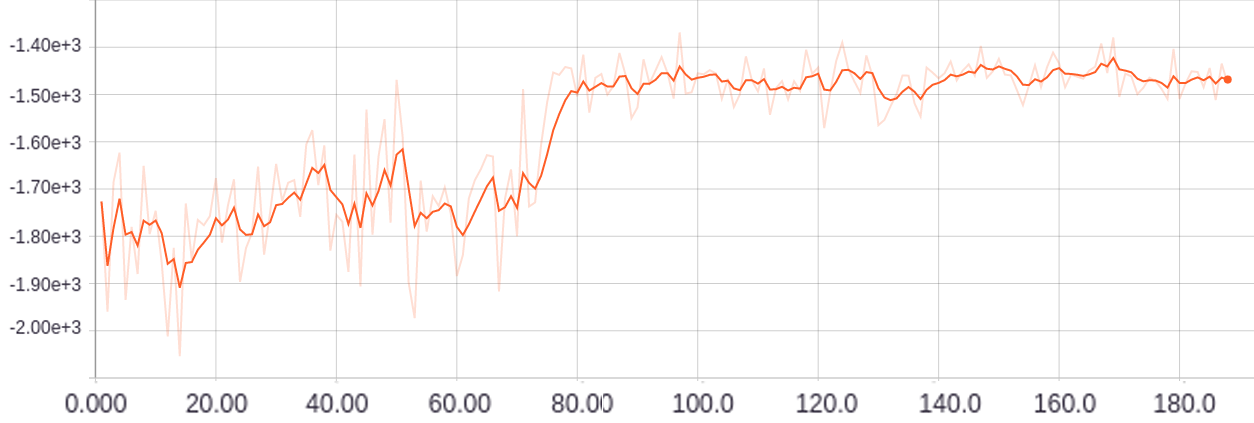
\includegraphics[width=14cm]{./img/optimiz}
  \caption{POIS optimization progress. On the $x$ axis is the number of iterations, on the $y$ axis is the mean value of the reward function for the sampled trajectories}
   \label{fig:poislearning}
\end{figure}

Fig.\ref{fig:means} and Fig.\ref{fig:means2} show the optimization progress of the hyperpolicy $\nu_{\boldsymbol \rho}$ with respect to the amount of sampled trajectory.
That is, Fig.\ref{fig:means} shows the learning progress of $\boldsymbol \omega$, which is the mean value of the parameter $\boldsymbol \rho$.
Fig.\ref{fig:means2} shows with a higher level of detail the progress of the means parameters $\alpha_1$,$\alpha_2$,$\alpha_3$, $\beta_1$, $\gamma_1$, which in Fig.\ref{fig:means} are too skewed to appreciate the differences.
The parameter $\boldsymbol \omega$ has been initialized with a vector $\boldsymbol \omega_0$ found with a trial-and-error approach.

\begin{figure}[H]
 \centering
  \captionsetup{width=10cm}
  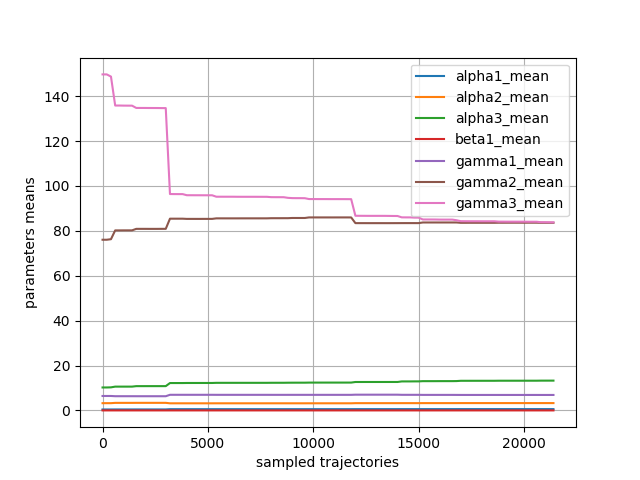
\includegraphics[width=10cm]{./img/parameters/means1}
  \caption{On the $x$ axis is the number of sampled trajectories; on the $y$ axis is the mean value of each parameter $\omega_i$}
   \label{fig:means}
\end{figure}

\begin{figure}[H]
 \centering
  \captionsetup{width=10cm}
  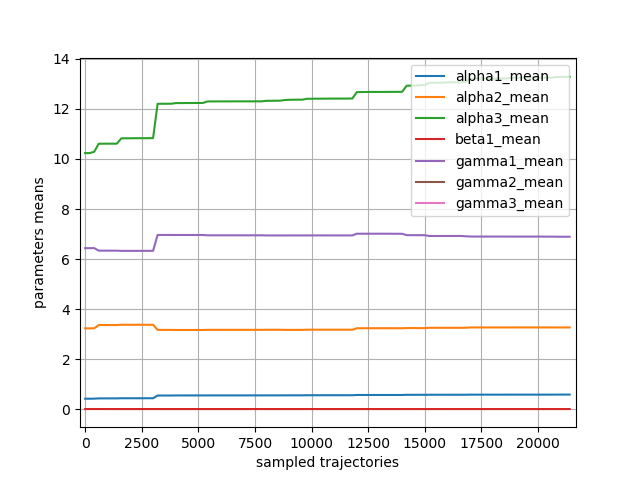
\includegraphics[width=10cm]{./img/parameters/means2}
  \caption{On the $x$ axis is the amount of sampled trajectories; on the $y$ axis is the mean value of each parameter $\omega_i$}
   \label{fig:means2}
\end{figure}


Fig.\ref{fig:log_stds} shows the progress of the standard deviations $\boldsymbol \sigma$. For a better visualization, we plotted the natural logarithm of the standard deviation instead of the std.
The parameter $\boldsymbol \sigma$ has been initialized with a vector $\boldsymbol \sigma_0= \boldsymbol 1.$ As expected, the standard deviations, as the number of sampled trajectories grow, tend to decrease. This means that the algorithm tends to explore less and less.


\begin{figure}[H]
 \centering
  \captionsetup{width=10cm}
  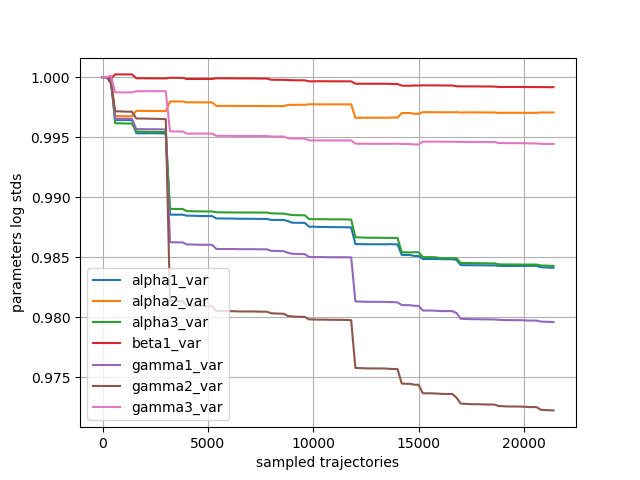
\includegraphics[width=10cm]{./img/parameters/log_stds}
  \caption{On the $x$ axis is the amount of sampled trajectories; on the $y$ axis is the logarithm of the standard deviation of each parameter $\omega_i$}
   \label{fig:log_stds}
\end{figure}



\subsubsection{Delta analysis}

The purpose of the rule-based policy $\psi_{\boldsymbol \omega}$ is to follow the reference trajectory. This translates into minimizing the difference between their position, velocity and orientation.
What follows shows the behavior of the optimal controller obtained by being trained with POIS, compared to the one fed with hand-tuned parameters, with respect to the reference trajectory.

\textbf{Delta position}
\label{sec:deltarho}
Fig.\ref{fig:delta_position} shows a comparison between the delta of the positions (i.e. the Euclidean distance) with respect to the reference trajectory along it, of the human-coded controller and the learned one.
As it can be noticed, the learned controller is almost always closer in the domain space to the reference trajectory with respect to the human one.

\begin{figure}[H]
 \centering
  \captionsetup{width=10cm}
  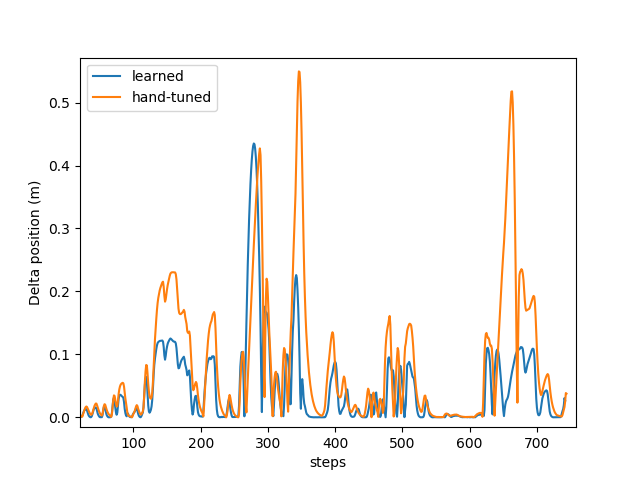
\includegraphics[width=10cm]{./img/deltas_pois/delta_position}
  \caption{On the $x$ axis are the steps of the trajectories, on the $y$ are the delta position, i.e. the 2D Euclidean distances between the reference trajectory and the two version of the controller.}
   \label{fig:delta_position}
 
Fig.\ref{fig:deltaposexpl} shows a detail of the comparison between the trajectories generated by the controller with human-crafted features and with a POIS learned policy with respect to the curves number 3 and 5. It can be noticed that in both these two curves the learned policy outperforms the hand-tuned one, following the reference trajectory with a higher level of accuracy.
 
\end{figure}
\begin{figure}[H]
\centering
\subfigure[Curve 3]
{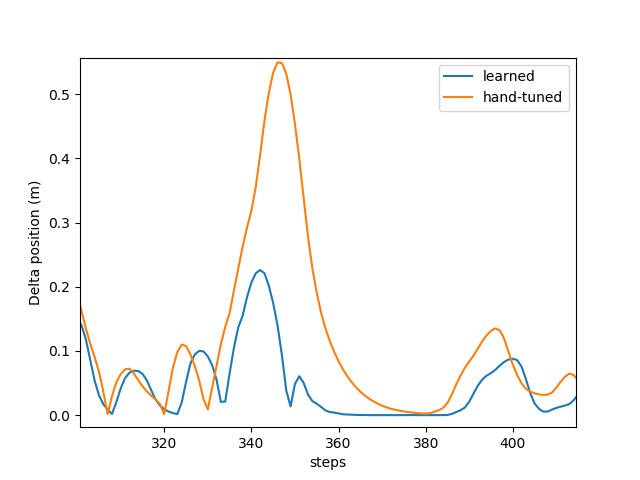
\includegraphics[width=6cm]{./img//deltas_pois/delta_rho_curva3}}
\hspace{3mm}
\subfigure[Curve 5]
{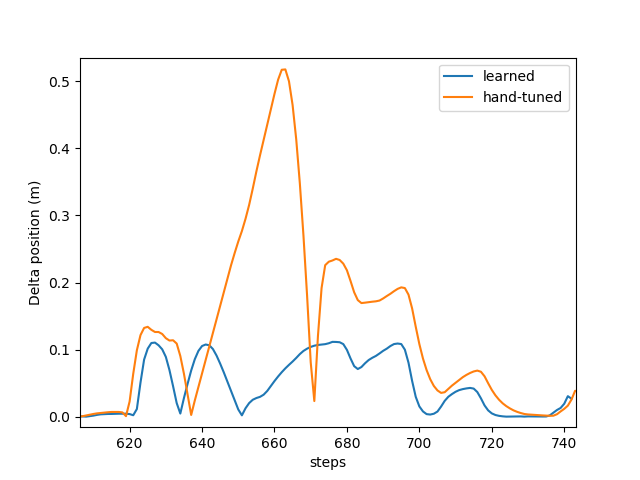
\includegraphics[width=6cm]{./img/deltas_pois/delta_rho_curva5}}
\caption{Detail of curves 3 and 5, with the comparison between the hand-tuned policy parameters and the learned policy parameters with respect to the reference trajectory concerning the position.}
\label{fig:deltaposexpl}
\end{figure}

In Fig.\ref{fig:curvespos}, this behaviour is show from the perspective of the absolute coordinates $(x,y)$.




\begin{figure}[H]
\centering
\subfigure[Curve 3]
{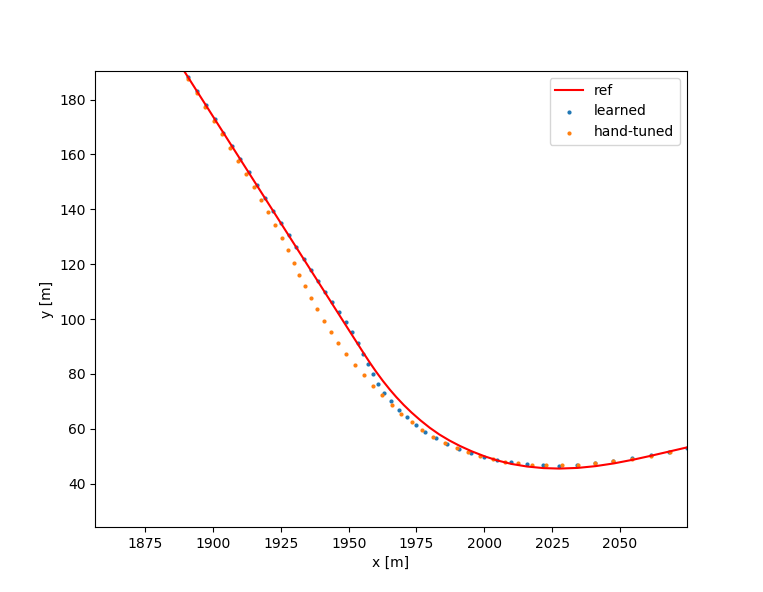
\includegraphics[width=7cm]{./img/traj_map/curve3}}
\hspace{2mm}
\subfigure[Curve 5]
{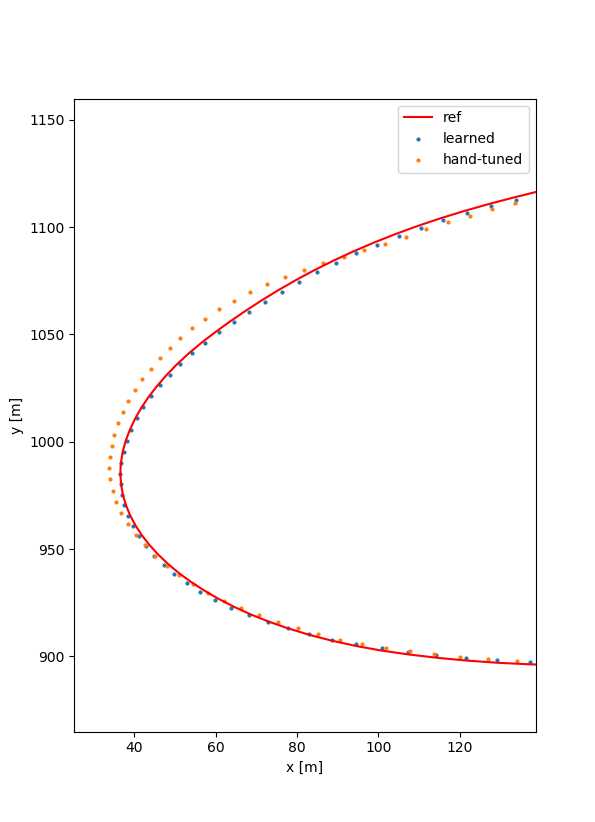
\includegraphics[width=5cm]{./img/traj_map/curve5}}
\caption{Detail of curves 3 and 5, with the comparison between the hand-tuned policy parameters and the learned policy parameters with respect to the reference trajectory, regarding the coordinates $(x,y)$.}
\label{fig:curvespos}
\end{figure}





\textbf{Delta velocity}
What follows are the results of the minimization of the difference of the rule-based policy and the reference trajectory concerning the speed. In particular, we focus on the longitudinal velocity, which is more meaningful for the lap-time metrics.
In Fig.\ref{fig:delta_vx} is represented the difference between the longitudinal velocities of the learned and human controller with respect with the reference trajectory. In Fig.\ref{fig:deltavxexpl} are the details on the curve 2 and 5.


\begin{figure}[H]
 \centering
  \captionsetup{width=10cm}
  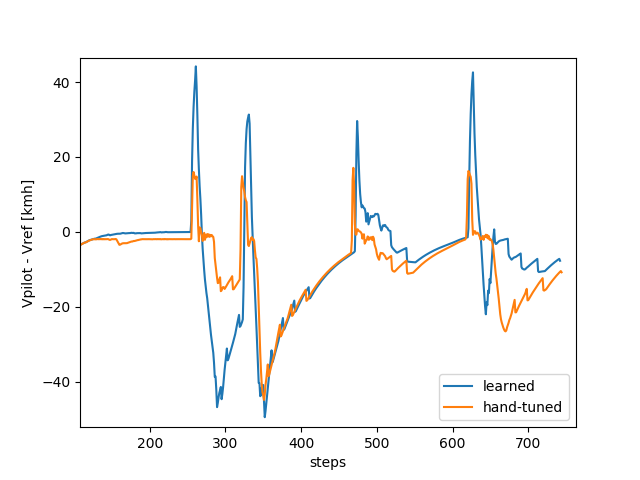
\includegraphics[width=10cm]{./img/deltas_pois/delta_vx}
  \caption{Full lap plot of the speed along the reference trajectory, the learned policy and the hand-tuned parameters.  On the $x$ axis are the trajectory steps; on the $y$ axis is the speed of the car.}
   \label{fig:delta_vx}
\end{figure}

\begin{figure}[H]
\centering
\subfigure[Curve 2]
{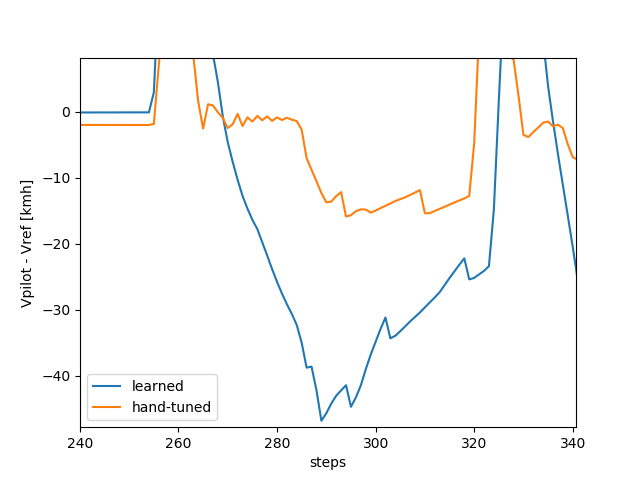
\includegraphics[width=6cm]{./img/deltas_pois/delta_vx_curva2}}
\hspace{3mm}
\subfigure[Curve 5]
{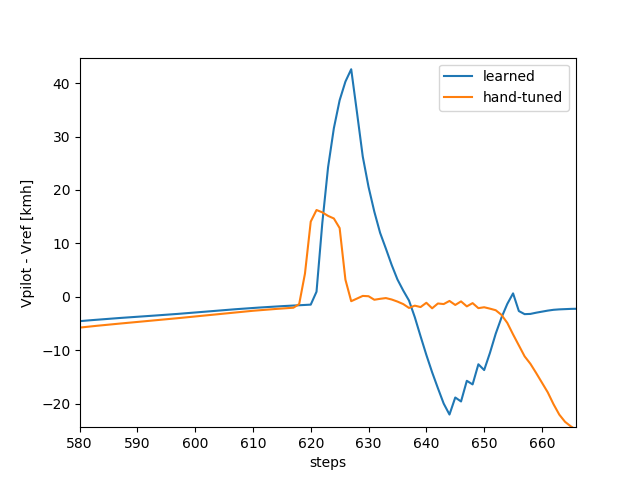
\includegraphics[width=6cm]{./img/deltas_pois/delta_vx_curva5}}
\caption{Comparisons of the differences of the longitudinal velocities between the reference trajectory and two policies: one with the learned parameters, the other with the hand-tuned parameters. On the $x$ axis are the trajectory steps; on the $y$ axis is the longitudinal velocities.}
\label{fig:deltavxexpl}
\end{figure}


Fig.\ref{fig:Vx} shows the behaviour of the policy from the point of view of the longitudinal velocity $v_x$.
In particular, Fig.\ref{fig:vxexpl} shows in detail the behaviors in curve 2 and 5 with respect to the reference trajectory regarding the speed. These behaviors especially occur in the curves, where the controller with the learned parameters runs at a lower speed with respect to the hand-tuned parameters. This behavior results effective for better following the reference trajectory position. In fact, as it can be seen in Table \ref{tab:avgspeed}, the average speeds of the learned parameters policy is slightly better than the hand-tuned one, because the lower speed on the corners allows to travel a lower distance, as also seen in Section \ref{sec:deltarho}

\begin{figure}[H]
 \centering
  \captionsetup{width=10cm}
  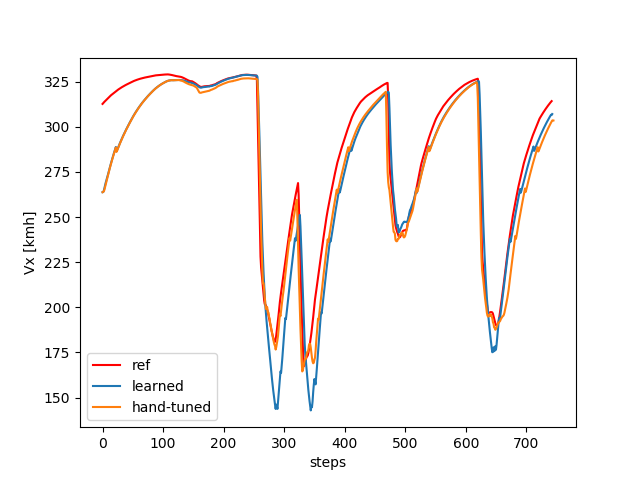
\includegraphics[width=10cm]{./img/velocities_pois/speed_x_comparison}
  \caption{On the $x$ axis are the steps of the trajectories, on the $y$ delta of the longitudinal velocity of human and learned controller with respect to the reference trajectory.}
   \label{fig:Vx}
\end{figure}

\begin{figure}[H]
\centering
\subfigure[Curve 2]
{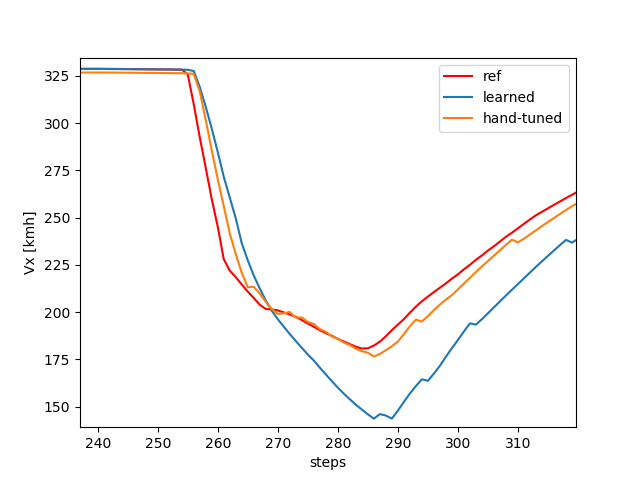
\includegraphics[width=6cm]{./img/velocities_pois/vx_curva2}}
\hspace{3mm}
\subfigure[Curve 5]
{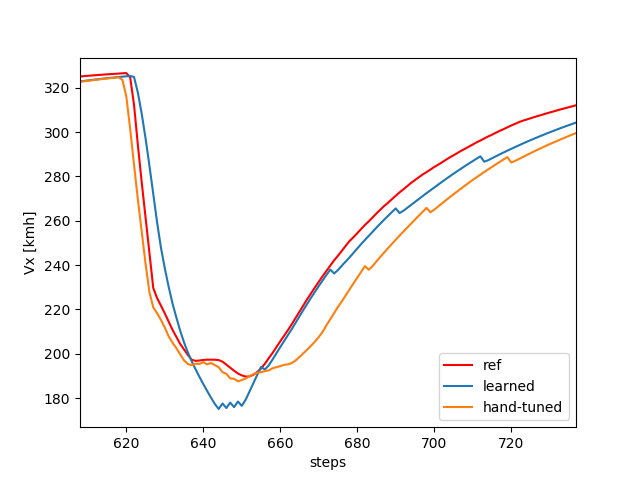
\includegraphics[width=6cm]{./img/velocities_pois/vx_curva5_rettilineo_finale}}
\caption{Detail of curves 2 and 5, with the comparison between the hand-tuned policy parameters and the learned policy parameters with respect to the reference trajectory concerning the longitudinal velocity.}
\label{fig:vxexpl}
\end{figure}

\begin{table}[H]
\centering
\begin{tabular}{|c|c|}
\hline
\textbf{Driver}                                                                      & \textbf{Average Lap-Speed (kmh)} \\ \hline
Reference  Trajectory   & 288.13                 \\ \hline
\begin{tabular}[c]{@{}c@{}}Controller\\  (Human Crafted Parameter)\end{tabular}      & 277.38                 \\
\hline
\begin{tabular}[c]{@{}c@{}}Controller\\  (Learned Parameters with POIS)\end{tabular} & 277.96     \\ \hline           
\end{tabular}
\caption{Average speed to complete a lap.}
\label{tab:avgspeed}
\end{table}

\textbf{Delta Orientation}

In Fig. \ref{fig:deltaorien} we show the orientation differences of curve number 2 and 5. It can be noticed that the controller with the two different sets of parameters does not show big discrepancy, but in some cases it results been more stable.

\begin{figure}[H]
\centering
\subfigure[Curve 2]
{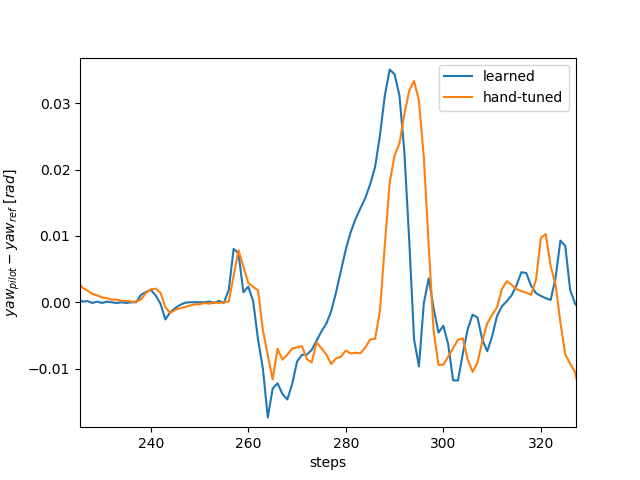
\includegraphics[width=6cm]{./img/deltas_pois/delta_orientation_curva2}}
\hspace{3mm}
\subfigure[Curve 5]
{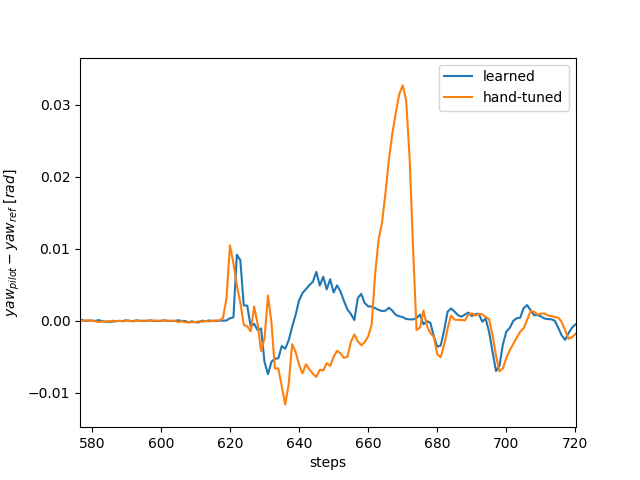
\includegraphics[width=6cm]{./img/deltas_pois/delta_orientation_curva5}}
\caption{Comparisons of the differences of orientations between the reference trajectory and two policies: one with the learned parameters, the other with the hand-tuned parameters. On the $x$ axis are the trajectory steps; on the $y$ axis is the delta orientation.}
\label{fig:deltaorien}
\end{figure}


In Fig.\ref{fig:laptime_pois} is shown the progress of the lap-time obtained with the rule-based policy $\psi_{\boldsymbol \omega}$ optimizing with POIS.
As expected, a rule-based policy itself cannot outperform the expert's performance. In fact, at converge, i.e. at the optimal delta minimization, not only it does not obtain a better lap-time with respect to the reference trajectory (see Table \ref{table:controller_lap_time}), but it is not even the best it obtains along its learning process.


\begin{figure}[H]
 \centering
  \captionsetup{width=10cm}
  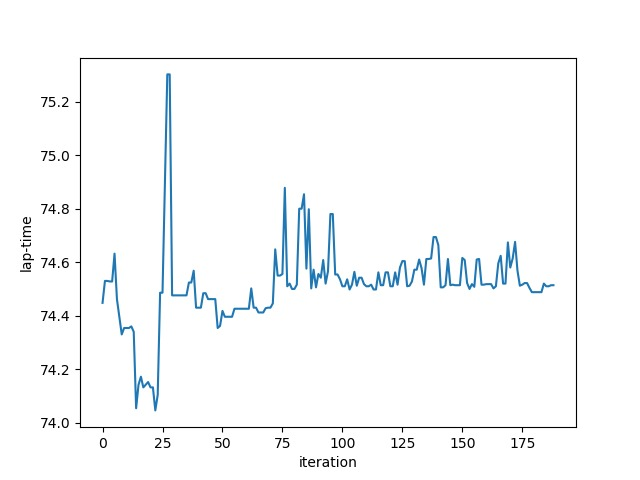
\includegraphics[width=10cm]{./img/means-lap-time}
  \caption{On the $x$ axis is the amount of sampled trajectories; on the $y$ axis is the logarithm of the standard deviation of each parameter $\omega_i$}
   \label{fig:laptime_pois}
\end{figure}





\begin{table}[H]
\centering
\begin{tabular}{|c|c|}
\hline
\textbf{Driver}                                                                      & \textbf{Lap-time (s)} \\ \hline
Reference  Trajectory   & 71.99                 \\ \hline
\begin{tabular}[c]{@{}c@{}}Controller\\  (Human Crafted Parameter)\end{tabular}      & 74.50                 \\
\hline
\begin{tabular}[c]{@{}c@{}}Controller\\  (Learned Parameters with POIS)\end{tabular} & 74.45     \\ \hline           
\end{tabular}
\caption{Best lap-time obtained by each algorithm with respect to the reference trajectory}
\label{table:controller_lap_time}
\end{table}


Concluding, the controller optimized with POIS behaves as expected, being able to follow the reference trajectory with a satisfying degree of accuracy.
However, it shows some deviating behaviours with respect to the reference trajectory regarding the speed. These behaviors especially occur in the curves, where the controller with the learned parameters runs at a lower speed with respect to the hand-tuned parameters. 


\section{Action Analysis}

\textbf{Throttle}
\begin{figure}[H]
 \centering
  \captionsetup{width=10cm}
  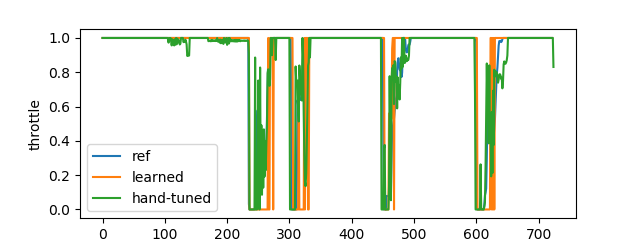
\includegraphics[width=10cm]{./img/action_pois/throttle}
  \caption{On the $x$ axis are the steps of the trajectories, on the $y$ delta of the longitudinal velocity of human and learned controller with respect to the reference trajectory.}
   \label{fig:throttle}
\end{figure}

\begin{figure}[H]
\centering
\subfigure[Curve 2]
{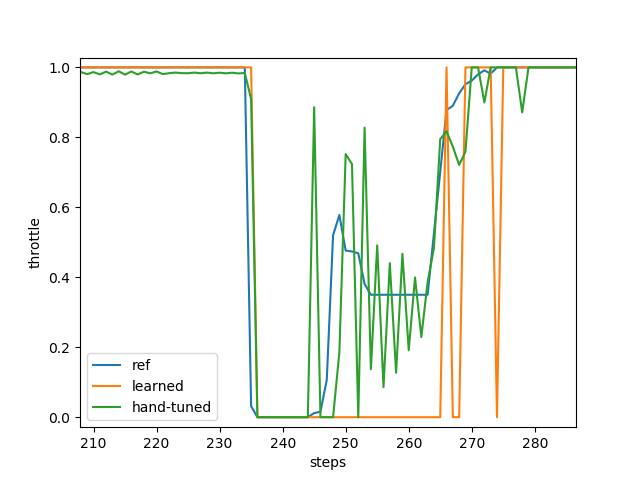
\includegraphics[width=6cm]{./img/action_pois/throttle_curva2}}
\hspace{1mm}
\subfigure[Curve 3]
{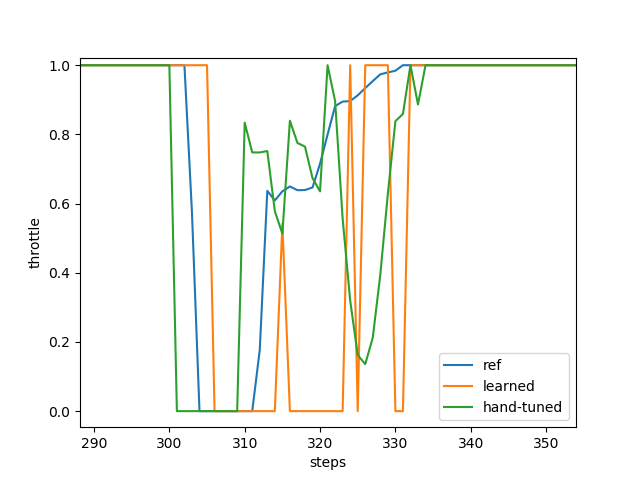
\includegraphics[width=6cm]{./img/action_pois/throttle_curva3}}
\hspace{1mm}
\subfigure[Curve 4]
{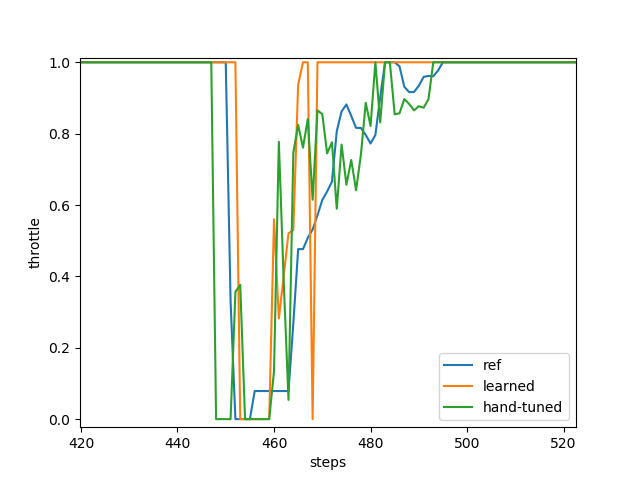
\includegraphics[width=6cm]{./img/action_pois/throttle_curva4}}
\hspace{1mm}
\subfigure[Curve 5]
{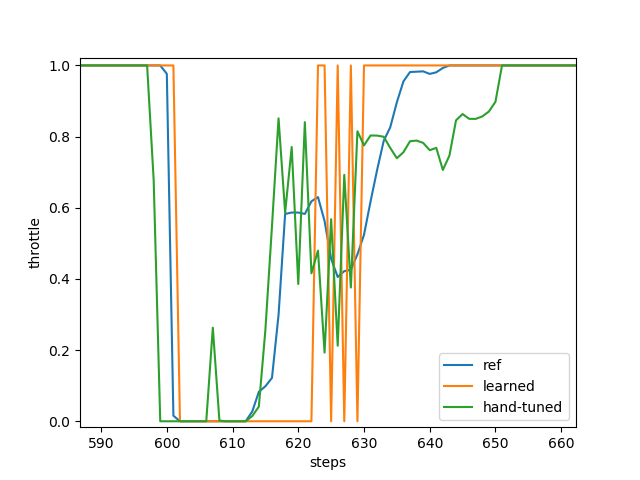
\includegraphics[width=6cm]{./img/action_pois/throttle_curva5}}
\caption{Comparisons of the differences of orientations between the reference trajectory and two policies: one with the learned parameters, the other with the hand-tuned parameters. On the $x$ axis are the trajectory steps; on the $y$ axis is the delta orientation.}
\label{fig:throttleexpl}
\end{figure}

\begin{figure}[H]
 \centering
  \captionsetup{width=10cm}
  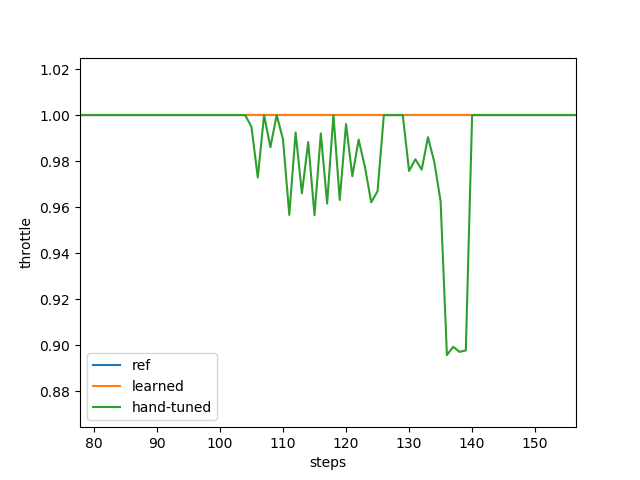
\includegraphics[width=10cm]{./img/action_pois/throttle_rettilineo}
  \caption{On the $x$ axis is the amount of sampled trajectories; on the $y$ axis is the logarithm of the standard deviation of each parameter $\omega_i$}
   \label{fig:throttleexplrett}
\end{figure}





\textbf{Brake}
\begin{figure}[H]
\hspace*{-1cm}
 \centering
  \captionsetup{width=10cm}
  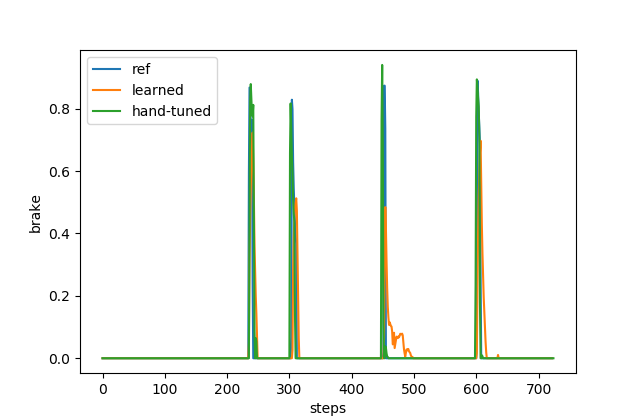
\includegraphics[width=10cm]{./img/action_pois/brake}
  \caption{On the $x$ axis are the steps of the trajectories, on the $y$ delta of the longitudinal velocity of human and learned controller with respect to the reference trajectory.}
   \label{fig:brake}
\end{figure}

\begin{figure}[H]
\centering
\subfigure[Curve 2]
{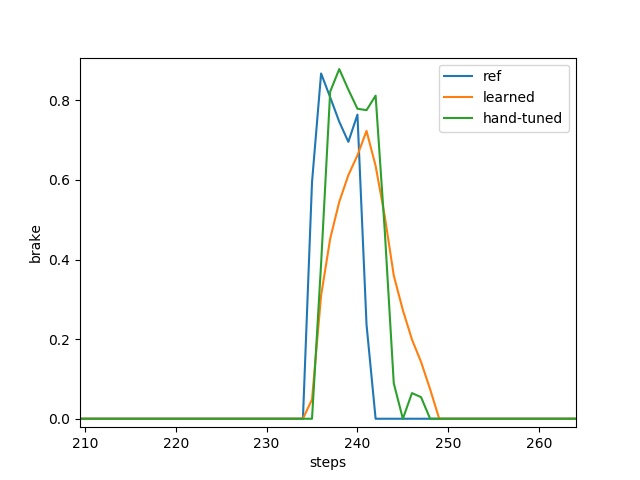
\includegraphics[width=6cm]{./img/action_pois/brake_human_curva2}}
\hspace{1mm}
\subfigure[Curve 3]
{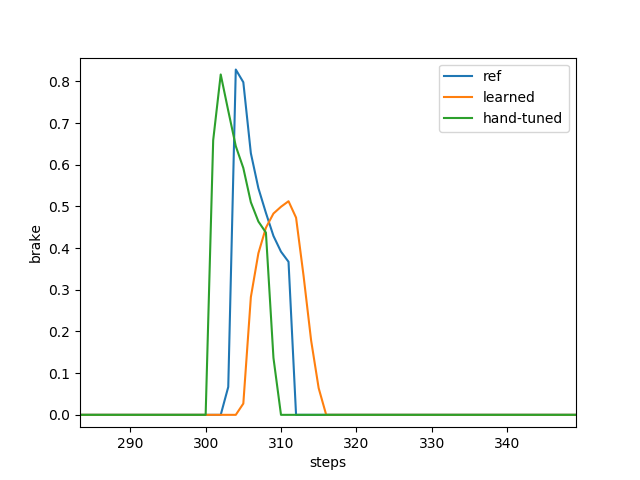
\includegraphics[width=6cm]{./img/action_pois/brake_human_curva3}}
\hspace{1mm}
\subfigure[Curve 4]
{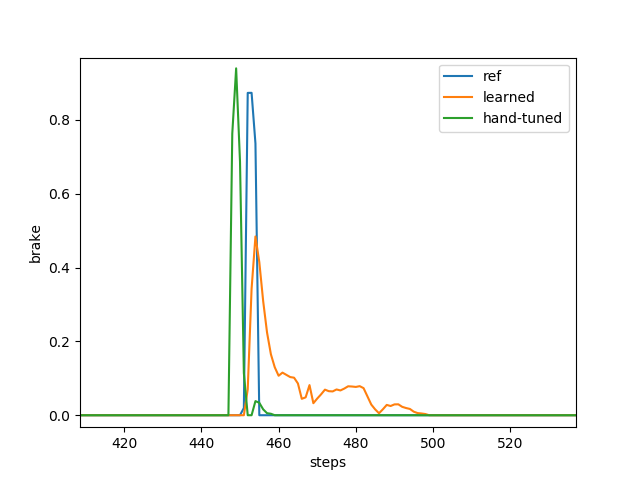
\includegraphics[width=6cm]{./img/action_pois/brake_human_curva4}}
\hspace{1mm}
\subfigure[Curve 5]
{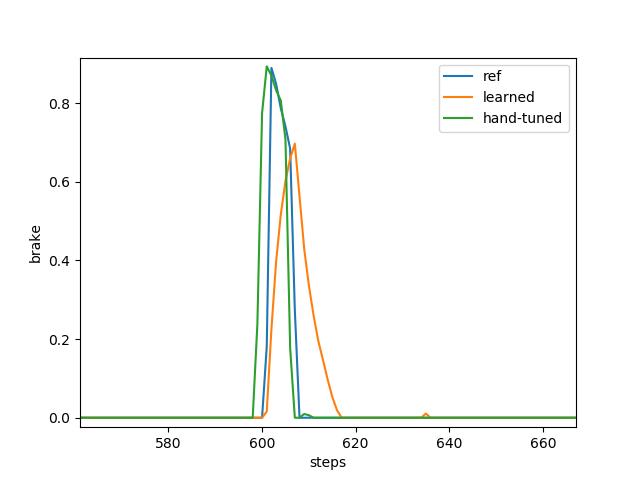
\includegraphics[width=6cm]{./img/action_pois/brake_human_curva5}}
\caption{Comparisons of the differences of orientations between the reference trajectory and two policies: one with the learned parameters, the other with the hand-tuned parameters. On the $x$ axis are the trajectory steps; on the $y$ axis is the delta orientation.}
\label{fig:brakeexpl}
\end{figure}


\textbf{Steer}
\begin{figure}[H]
 \centering
  \captionsetup{width=10cm}
  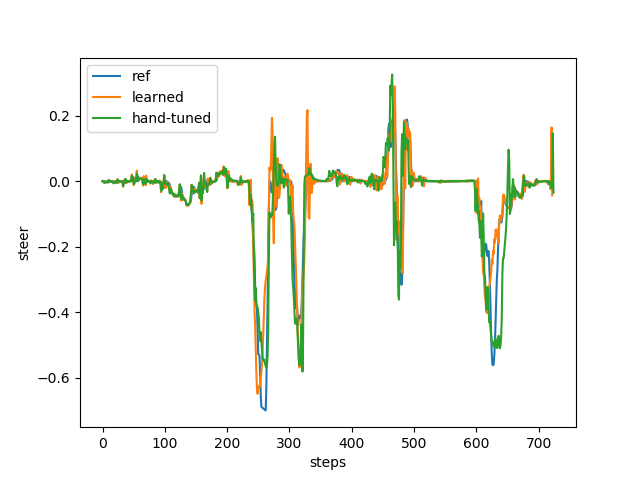
\includegraphics[width=10cm]{./img/action_pois/steer}
  \caption{On the $x$ axis are the steps of the trajectories, on the $y$ delta of the longitudinal velocity of human and learned controller with respect to the reference trajectory.}
   \label{fig:steer}
\end{figure}





\subsection{PPO}





